\section{ADMIT Tools}

This section shows some of the tools that we have
been prototyping for ADMIT. The tool are layered on top
of the XML infrastructure of ADMIT and  communicate through
that sturcture for inputs and outputs. We envision
that there will be a set of basic tools that create some
of the Basic Data Products and there will be an evolving
set of tool that add new capability. The tools will be
compatable with the CASA environment and utilize the CASA
core and existing CASA routines where applicable. The tools
will operate on CASA image format data.

A second operational goal for tools is that they can
be re-executed based on data in the ADMIT XML files and the
XML files can be modified to allow the tools to be re-run
in bulk. For example, if you decide to change the velocity
range for a moment map, you could modify the XML information
and then re-run the moments for all of the lines of interest with
with a single command.

\subsection{Line Identification and Line Cutout}

The Line ID Tool will compare the rest frequency coverage of the 
image cubes with a database of common line retrieved from Splatalogue to 
identify the appropriate channel/cube locations of potential lines.  
A line-strength vs. frequency table is the essential input into a line 
identification procedure (here we will leverage Tony Remijan’s datasplat project). 
The input data for the procedure will be improved by the previously computed 
per-channel cube statistics and aided by cross-correlation techniques in a 
position-velocity diagram (Figure 7) or in the cube itself. The output will 
be a series of identified and unidentified lines across the different bands 
in a simple table of line, frequency, channel range, and detection probability.

\begin{figure}[t]
\centering
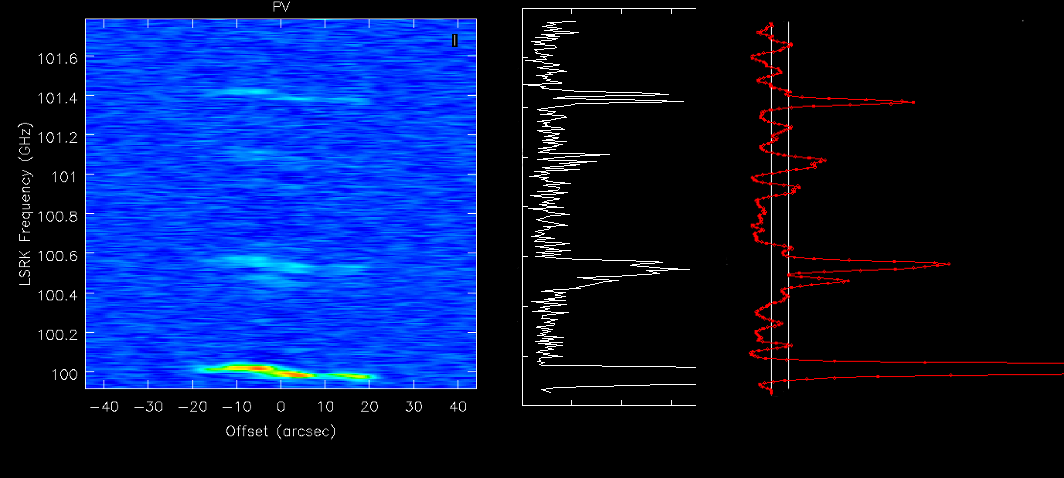
\includegraphics[width=0.75\textwidth]{line-id.png}
\hspace{0.03in}
\caption{\small \setlength{\baselineskip}{0.85\baselineskip}
Line identification can be tremendously improved in a position-velocity diagram
by cross-correlating the signal in the velocity direction. In Figure 7, compare the more
traditional noisy peak/RMS plot in the middle (white) with the smooth
cross correlation technique on the right (in red). The lines are better
resolved using the cross-correlation technique. The two vertical lines
denote zero (white line) and a 3-sigma clipping (gray line).
  }
  \label{fig:hst}
  \end{figure}


Based on the line identification line tables, line cutout cubes can be 
extracted, with now the third axis in Doppler velocity space, to ensure that 
we can compare the different lines and molecules on the same basis. Depending 
on the number of lines in the bands, keeping only the line cubes can significantly 
cut down user disk usage.

\subsection{Moment Maps}

Moment maps are a simple, yet powerful tool for examining global properties 
of an object’s emission. The most commonly used maps are integrated flux 
(moment 0), centroid velocity (moment 1), and velocity dispersion (moment 2).  
The Moment Map tool takes the line cubes produced by the Line ID Tool and 
creates the three moment maps for each spectral line (see Figure 8). The moment 
can be clipped based on simple RMS cutoff (already computed by the Data 
Summary tool!), but also could employ more sophisticated methods such as local 
smoothing to increase the signal to noise to create a more robust clipping mask. 
Moment maps can also be produced using parametric shapes, e.g. a Gaussian fit, 
which would then store the total emission, mean velocity and width of the 
spectrum at each location.

The advantage of the ADMIT approach is that the previous steps of line definition
and rest frequency assignment allow automated calculation of the velocity scale
for each line. This can be combined with simple spectra at peak position as
shown in the mock-up figure.

\begin{figure}[t]
\centering
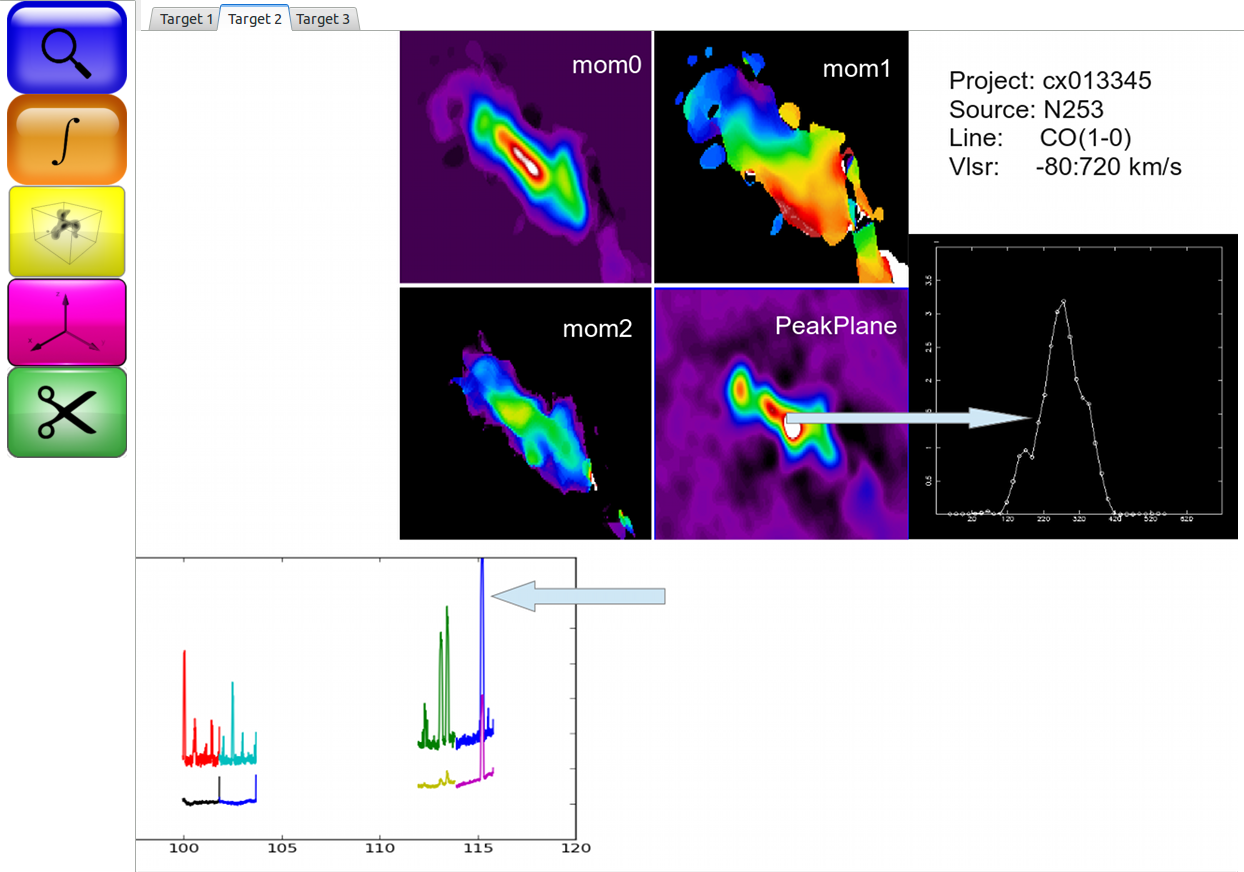
\includegraphics[width=0.75\textwidth]{moments.png}
\hspace{0.03in}
\caption{\small \setlength{\baselineskip}{0.85\baselineskip}
Mockup of the detailed view of some of the data products of a 
single source and spectral line, as produced by the Data Summary tool \
for the target source selected in the middle panel. In this scenario, 
the user has clicked on the CO data cube icon in Figure 6. 
On the top row, tabs are visible for a number of collected sources. 
The lower arrow indicates which line is the CO line in the full-band 
spectra. The upper arrow indicates the reference position for the spectrum shown.
  }
 \label{fig:moments}
\end{figure}
